\documentclass[a4paper]{article}

\usepackage{inputenc}
\usepackage[british,UKenglish]{babel}
\usepackage{amsmath}
%\usepackage{titlesec}
\usepackage{color}
\usepackage{graphicx}
\usepackage{fancyref}
\usepackage{hyperref}
\usepackage{float}
\usepackage{scrextend}
\usepackage{setspace}
\usepackage{xargs}
\usepackage{multicol}
\usepackage{nameref}

\usepackage{sectsty}
\usepackage{multicol}
\usepackage{multirow}
\usepackage[procnames]{listings}
\usepackage{appendix}

\newcommand\tab[1][1cm]{\hspace*{#1}}
\hypersetup{colorlinks=true, linkcolor=black}
\interfootnotelinepenalty=10000

\newcommand{\cleancode}[1]{\begin{addmargin}[3em]{3em}\texttt{\textcolor{cleanOrange}{#1}}\end{addmargin}}
\newcommand{\cleanstyle}[1]{\text{\textcolor{cleanOrange}{\texttt{#1}}}}


\usepackage[colorinlistoftodos,prependcaption,textsize=footnotesize]{todonotes}
\newcommandx{\commred}[2][1=]{\textcolor{Red}
{\todo[linecolor=red,backgroundcolor=red!25,bordercolor=red,#1]{#2}}}
\newcommandx{\commblue}[2][1=]{\textcolor{Blue}
{\todo[linecolor=blue,backgroundcolor=blue!25,bordercolor=blue,#1]{#2}}}
\newcommandx{\commgreen}[2][1=]{\textcolor{OliveGreen}{\todo[linecolor=OliveGreen,backgroundcolor=OliveGreen!25,bordercolor=OliveGreen,#1]{#2}}}
\newcommandx{\commpurp}[2][1=]{\textcolor{Plum}{\todo[linecolor=Plum,backgroundcolor=Plum!25,bordercolor=Plum,#1]{#2}}}

\def\code#1{{\tt #1}}

\def\note#1{\noindent{\bf [Note: #1]}}

\makeatletter
%% The "\@seccntformat" command is an auxiliary command
%% (see pp. 26f. of 'The LaTeX Companion,' 2nd. ed.)
\def\@seccntformat#1{\@ifundefined{#1@cntformat}%
   {\csname the#1\endcsname\quad}  % default
   {\csname #1@cntformat\endcsname}% enable individual control
}
\let\oldappendix\appendix %% save current definition of \appendix
\renewcommand\appendix{%
    \oldappendix
    \newcommand{\section@cntformat}{\appendixname~\thesection\quad}
}
\makeatother


% "define" Scala
\usepackage[T1]{fontenc}  
\usepackage[scaled=0.82]{beramono}  
\usepackage{microtype} 

\sbox0{\small\ttfamily A}
\edef\mybasewidth{\the\wd0 }

\lstdefinelanguage{scala}{
  morekeywords={abstract,case,catch,class,def,%
    do,else,extends,false,final,finally,%
    for,if,implicit,import,match,mixin,%
    new,null,object,override,package,%
    private,protected,requires,return,sealed,%
    super,this,throw,trait,true,try,%
    type,val,var,while,with,yield},
  sensitive=true,
  morecomment=[l]{//},
  morecomment=[n]{/*}{*/},
  morestring=[b]",
  morestring=[b]',
  morestring=[b]"""
}

\usepackage{color}
\definecolor{dkgreen}{rgb}{0,0.6,0}
\definecolor{gray}{rgb}{0.5,0.5,0.5}
\definecolor{mauve}{rgb}{0.58,0,0.82}

% Default settings for code listings
\lstset{frame=tb,
  language=scala,
  aboveskip=3mm,
  belowskip=3mm,
  showstringspaces=false,
  columns=fixed, % basewidth=\mybasewidth,
  basicstyle={\small\ttfamily},
  numbers=none,
  numberstyle=\footnotesize\color{gray},
  % identifierstyle=\color{red},
  keywordstyle=\color{blue},
  commentstyle=\color{dkgreen},
  stringstyle=\color{mauve},
  frame=single,
  breaklines=true,
  breakatwhitespace=true,
  procnamekeys={def, val, var, class, trait, object, extends},
  procnamestyle=\ttfamily\color{red},
  tabsize=2
}

\lstnewenvironment{scala}[1][]
{\lstset{language=scala,#1}}
{}
\lstnewenvironment{cpp}[1][]
{\lstset{language=C++,#1}}
{}
\lstnewenvironment{bash}[1][]
{\lstset{language=bash,#1}}
{}
\lstnewenvironment{verilog}[1][]
{\lstset{language=verilog,#1}}
{}



\lstset{frame=, basicstyle={\footnotesize\ttfamily}}

\graphicspath{ {images/} }
\usepackage{ctex}
\usepackage{verbatim}
\usepackage{enumerate}
\usepackage{geometry}
\usepackage{amssymb}
\usepackage{amsmath}
%\usepackage{slashbox}
\usepackage{diagbox}
\usepackage{pifont}%\ding{192} \ding{172}
\usepackage{tikz}
\usepackage{booktabs}
\usepackage{float}
\usepackage{bm}
\usepackage{siunitx}
%\geometry{a4paper, scale=0.72}
\geometry{a4paper,left=2.5cm,right=2.5cm,top=2.5cm,bottom=2.5cm}
%%%%%%%%%%%%%%%%%%%%%%%%%%%%%%%%%%%%%%%% BEGIN DOC %%%%%%%%%%%%%%%%%%%%%%%%%%%%%%%%%%%%%%%%

\begin{document}
\setlength{\abovecaptionskip}{0pt}
\setlength{\belowcaptionskip}{0pt}
\renewcommand{\contentsname}{目\ 录}
\renewcommand{\appendixname}{附录}
\renewcommand{\appendixpagename}{附录}
\renewcommand{\refname}{参考文献} 
\renewcommand{\figurename}{图}
\renewcommand{\tablename}{表}
\renewcommand{\today}{\number\year 年 \number\month 月 \number\day 日}
\newcommand{\refeq}[1]{\textbf{Eq.(\ref{#1})}}
\newcommand*{\circled}[1]{\lower.7ex\hbox{\tikz\draw (0pt, 0pt)%
    circle (.5em) node {\makebox[1em][c]{\small #1}};}}
\title{{\Huge 近代物理实验报告{\large\linebreak\\}}{\Large 实验7-2:\ 用传输式谐振腔观测铁磁共振\linebreak\linebreak}}
%please write your name, Student #, and Class # in Authors, student ID, and class # respectively
\author{\\姓\ 名:付\ 大\ 为\\
学\ 号: 1800011105\\
邮\ 箱: \url{fudw@pku.edu.cn}\\
%班\ 号: xxxxx\\\\
近代物理实验 (II)\\
(2022,春季学期)\\\\
北京大学\\
物理学院\\
2018级1班}
\date{\today}
\maketitle
\newpage

%%%%%%%%%%%%%%%%%%%%%%%%%%%%%%%%%%%%%%%% ABSTRACT %%%%%%%%%%%%%%%%%%%%%%%%%%%%%%%%%%%%%%%%
\begin{center}
{\Large\bf{摘\ 要\\}}
\end{center}

谐振腔是常用的微波元件之一,在微波技术中一般用作谐振腔波长计、微波电子管的组成部分或测量腔等.通过实验要求对谐振腔的结构、谐振条件、振荡模式和品质因数等有一定的了解.微波磁共振是微波与物质相互作用所发生的物理现象,磁共振方法已被广泛用来研究物质的特性、结构和弛豫过程.铁磁共振具有磁共振的一般特性,而且效应显著,用简单装置就可以进行观测,实验中,我们将观测铁磁共振曲线,测量共振磁场和共振线宽,计算出材料的g因子和弛豫时间.\\\\
{\bf{关键词}:}微波, 铁磁共振, g因子, 弛豫时间
\newpage

%%%%%%%%%%%%%%%%%%%%%%%%%%%%%%%%%%%%%%%% CONTENT %%%%%%%%%%%%%%%%%%%%%%%%%%%%%%%%%%%%%%%%
\begin{center}
\tableofcontents\label{c}
\end{center}
\newpage

%%%%%%%%%%%%%%%%%%%%%%%%%%%%%%%%%%%%%%%% Introduction %%%%%%%%%%%%%%%%%%%%%%%%%%%%%%%%%%%%%%%%
\section{引言} \label{overview}%------------------------------
受目前可得到的磁感应强度的限制,磁共振所涉及的共振频率一般处于射频与微波频段。通常,当材料的磁化强度较小(比如核磁共振)或者当所用的磁场较弱时(比如光泵磁共振),
常用射频电磁波做磁共振的激励信号;但在铁磁和电子顺磁共振中,由于它们的磁矩较大,磁效应比较显著,一般采用频率较高的微波来观测其磁共振效应。因为在微波波段,其能量量级大约是$10^{-6}\sim 10^{-3}\rm eV$,许多原子和分子发射和吸收的电磁波的能量正好处在这个波段,所以,微波与物质相互作用时可以发生共振现象。

目前,产生微波的主要方法有微波固体振荡器(比如微波晶体管振荡器、体效应管振荡
器、雪崩二极管振荡器)和一些特殊的微波电子管(比如反射式速调管、磁控管和行波管等)。常用的小功率微波振荡器有反射式速调管和体效应管振荡器。体效应管振荡器是利用具有双能谷结构的半导体材料中的负阻特性而形成的电流振荡输出微波的,它具有体积小、重量轻、工作电压低的特点,自20世纪六十年代诞生以后,已经逐步代替了速调管。大功率的微波输出通常采用晶体管振荡器(最高功率可达几十瓦)和磁控管(功率可达数十千瓦到几兆瓦)。

铁磁共振是指铁磁体材料在受到相互垂直的稳恒磁场和交变磁场的共同作用时发生的共振现象,它可以用于测定铁磁体材料的 g 因子、共振线宽、弛豫时间等性质。

谐振腔是微波系统中的重要元件,它能将特定频率的微波限制在一定的几何空间内,也就是说,谐振腔具有储蓄电磁能量和实现频率选择的功能。微波波段的谐振腔按几何形状分类,有矩形谐振腔、圆形谐振腔、同轴谐振腔等,而按所使用的材料分类则有金属谐振腔、介质谐振腔等。本实验中采用的是传输式金属矩形谐振腔,它实际上就是一段矩形波导管,并在两端加上带耦合孔的短路金属板。在谐振腔中,由于导体壁可防止电磁波辐射,使电磁场局限在空腔内部并在腔内连续反射,如果波型和频率合适,就会产生驻波,即发生谐振现象。

通过本实验主要让学生了解微波体效应振荡器的工作原理,了解微波传输的基本原理、
方法和元件,掌握传输式谐振腔的工作特性,了解用谐振腔观察铁磁共振的基本原理和实验条件。

%%%%%%%%%%%%%%%%%%%%%%%%%%%%%%%%%%%%%%%% Theory %%%%%%%%%%%%%%%%%%%%%%%%%%%%%%%%%%%%%%%%
\newpage
\section{理论} \label{theory}%------------------------------
在铁磁体材料中,有许多自发磁化的小区域——磁畴,磁畴内的磁矩是有序排列的,一个磁畴内自发磁化强度的平均值可用$M_s$表示,不同磁畴的$M_s$方向是不一致的。由于铁磁体具有很大的磁化率(其$\chi$值可达$10-10^{-6}$ 量级,所以,只需加很小的外加磁场,就能够调整磁畴$M_s$的取向,使其饱和磁化。
当铁磁体同时受到两个相互垂直的磁场即恒定磁场$H_0$(沿 Z 轴)和微波交变磁场$h$ 的作用时,恒定磁场$H_0$使铁磁体饱和磁化,当磁化强度矢量$M_s$原来的平衡方向与 $H_0$有夹角
$\theta$时,$M_s$将围饶$H_0$进动,其频率为:
\begin{equation}\label{eq:1}
    \omega_0=\gamma H_0
\end{equation}
其中γ为铁磁体材料的旋磁比,即
\begin{equation}
    \gamma=g\frac{\mu_0}{2m}
\end{equation}
式中g为朗德因子,$\mu_0$为真空磁导率,e和m分别为电子电量和电子质量。

当固定铁磁体所处微波磁场的频率为$\omega_0$,改变稳恒磁场H的大小,当H满足式\refeq{eq:1}即发生所谓的铁磁共振现象,设此时$H=H_r$。发生共振时,磁导率张量对角元$\mu$的虚部$\mu^{\prime\prime}$与稳恒磁场$H$的关系曲线上将出现共振峰, $\mu^{\prime\prime}$的最大值$\mu^{\prime\prime}_r$所对应的磁场$H_r$称为共振磁场,$\mu^{\prime\prime}=\mu^{\prime\prime}_r/2$所对应的两点间的磁场间隔$|H_1-H_2|$称为铁磁共振线宽,记作$\Delta H$,并且$\mu^{\prime\prime}=\mu^{\prime\prime}_r$时, $P=P_r$;$\mu^{\prime\prime}=\mu^{\prime\prime}_r/2$时,$P=P_{1/2}$.由上式得
\begin{equation}
    P_{1/2}=\frac{4P_0}{(\sqrt{P/P_0}+1)^2}
\end{equation}
弛豫时间满足
\begin{equation}
    \tau=\frac{2}{\gamma\Delta H}
\end{equation}
	

%%%%%%%%%%%%%%%%%%%%%%%%%%%%%%%%%%%%%%%% Experiment %%%%%%%%%%%%%%%%%%%%%%%%%%%%%%%%%%%%%%%%
\newpage
\section{实验} \label{experiment}%------------------------------

\subsection{实验仪器}
\begin{enumerate}[(1)]
    \item 速调管电源
    \item 速调管
    \item 隔离器
    \item 定向耦合器
    \item 吸收式波长计
    \item 晶体检波接头
    \item 可变衰减器
    \item 隔离器
    \item 谐振腔
    \item 样品
    \item 电磁铁
    \item 直流电源
    \item 电流表
    \item 检流计
\end{enumerate}

\begin{comment}
\subsection{简要实验步骤}\label{sub:ExperimentalSteps}
\begin{enumerate}[1.]
    \item 连接实验装置.先用脉冲发生器作输入信号源,用示波器观察各级输出,调节放大倍数,使得线性放大器输出的脉冲幅度为5~6V.
    \item 用示波器观察
    \item
    \item
\end{enumerate}

\circled{1}抽真空(按橘色按钮),约2分钟,机械泵声音平稳即可\\\\
\end{comment}
%%%%%%%%%%%%%%%%%%%%%%%%%%%%%%%%%%%%%%%% Results & Discussions %%%%%%%%%%%%%%%%%%%%%%%%%%%%%%%%%%%%%%%%
\newpage
\section{结果及分析}

%------------------------------------------------------------
\subsection{观测速调管的振荡模,测量一个振荡模的中心频率和电子调谐范围.}\label{sub1}
\begin{enumerate}[1)]
\item 观察速调管的振荡模,测量一个振荡模的中心频率和电子调谐范围.

最大电流刻度$I=\SI{50.0}{\mu A}$,中心频率$f_0=a+b\lambda=\SI{8319.50}{M\hertz}$,分别顺时针逆时针调节反射极旋钮,在电流读数为最大读数的一半时,用同上办法调节波长旋钮,记录对应的频率$f_1=\SI{9285.49}{M\hertz}$, $f_2=\SI{9341.47}{M\hertz}$,则电子调谐范围为
\begin{equation}
    |f_1-f_2|=\SI{55.98}{M\hertz}
\end{equation}
\item 观察传输式腔的谐振曲线,测量腔的有载品质因数.

检流计最大值所对应的格数$P=120$,$\lambda_0=3280$,中心频率$f_0=a+b\lambda_0=\SI{9321.82}{M\hertz}$;再分别顺时针和逆时针调节反射极旋钮,在检流计读数为最大读数的一半时,调节波长表旋钮,记录对应的频率,即$f_1=\SI{9320.13}{M\hertz}$,$f_2=\SI{9324.36}{M\hertz}$,则有载品质因数为
\begin{equation}
    Q=\frac{f_0}{|f_1-f_2|}=2203.74
\end{equation}
\end{enumerate}

%------------------------------------------------------------
\newpage
\subsection{观测铁磁共振}\label{sub2}
\begin{enumerate}[1)]
\item 用简便方法测量共振磁场$H_r$和线宽

记录检流计最大读数$P_{max}=120$,最小读数$P_r=60$,中点读数$P_{\frac{1}{2}}=90$,测量它们所对应的电流表读数如下\textbf{表~\ref{tab:table1}.}
\begin{table}[H]
\caption{\textbf{测量线宽$\Delta H$}}
\label{tab:table1}
\begin{center}
\setlength{\tabcolsep}{7mm}
\begin{tabular}{|c|c|c|c|c|c|}%p{6cm}|}
    \toprule
	\hline
	$\bm P_{\frac{1}{2}}$ & $\bm I_1/\si{A}$ & $\bm I_2/\si{A}$ & $\bm H_1/\si{Oe}$ & $\bm H_2/\si{Oe}$ & $\bm \Delta H/\si{Oe}$\\ \hline \hline
	90 & 2.131 & 2.401 & 3245 & 3650 & 405 \\ \hline
	90 & 2.123 & 2.433 & 3230 & 3655 & 425\\ \hline
	90 & 2.118 & 2.421 & 3230 & 3653 & 423\\ \hline
	\bottomrule
	\end{tabular}
\end{center}
\end{table}
查表得到$H_r=\SI{3448}{Oe}$,对表中$\Delta H$作平均得到$\Delta H=\SI{418}{Oe}$
\item 逐点绘制$P-H$曲线

改变变阻器的阻值,逐点测检流计读数$P$,以及对应的电流表示数I,直到检流计的读数再次稳定,测20到40个点.(注意由于磁滞效应,变阻器阻值只能向一个方向变动).查表得到H,绘制$P-H$曲线如下\textbf{图\ref{fig:fig1}}所示:
\begin{figure}[H]
 \centering
 \caption{$P-H$曲线}
 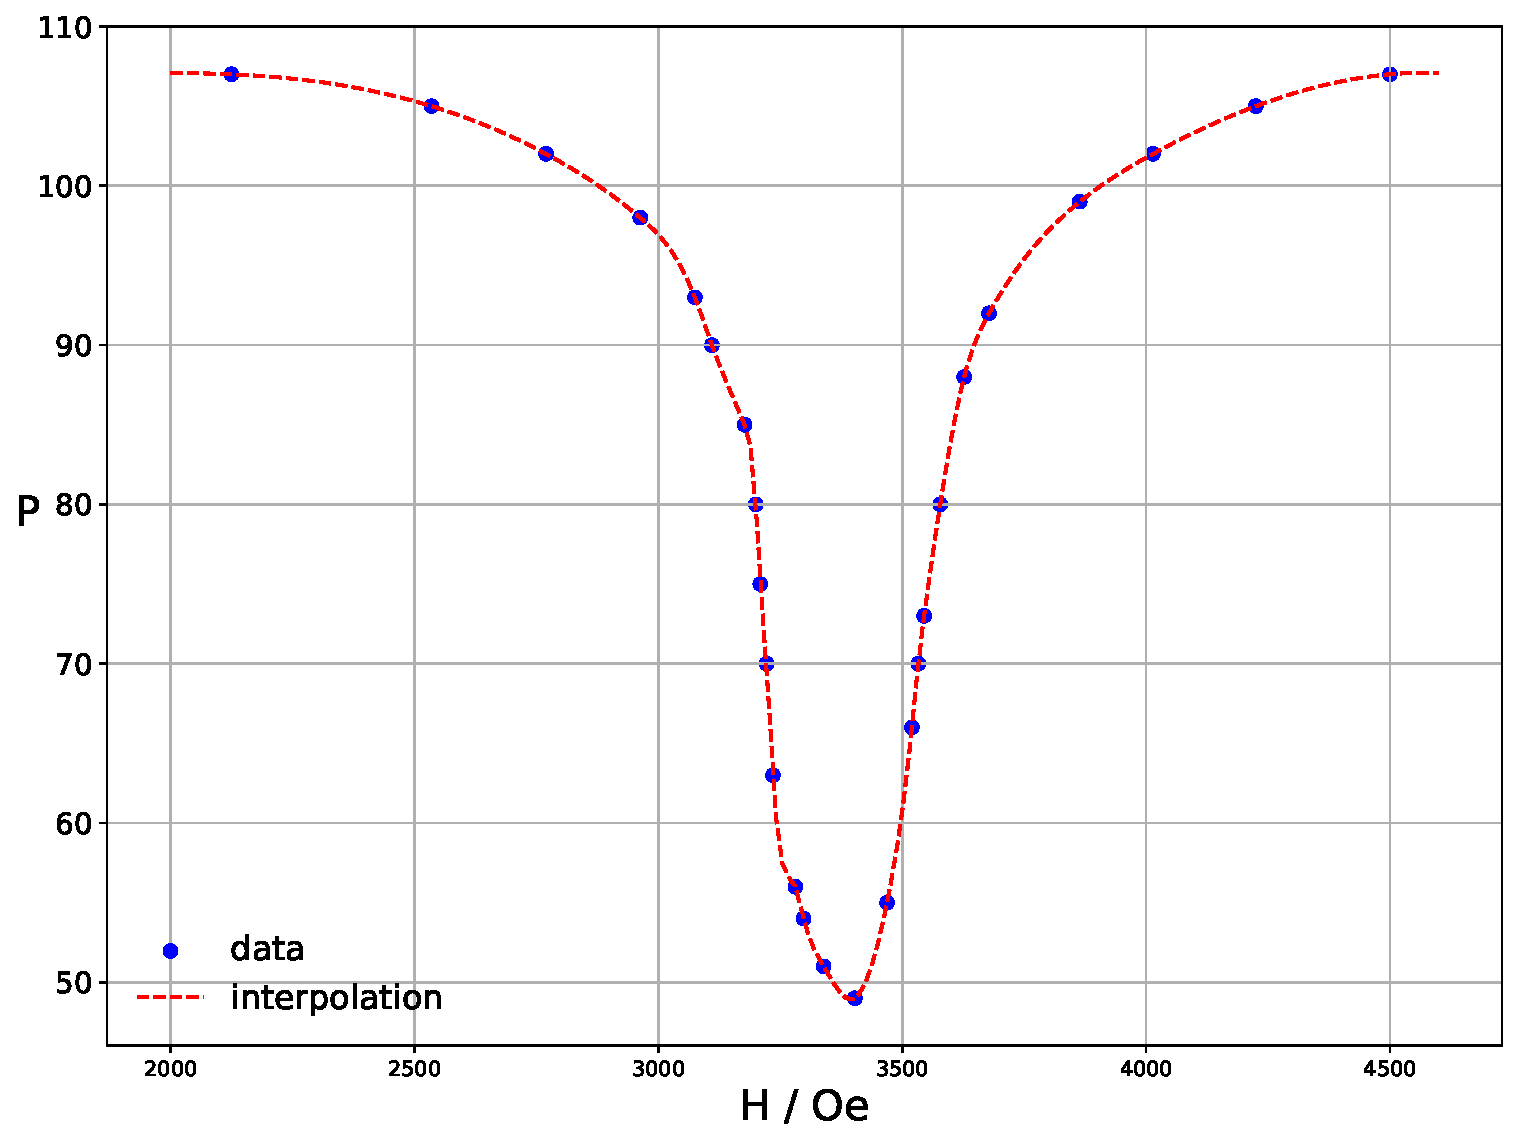
\includegraphics[height=11cm, width=15cm]{images/phyex1_fig.pdf}
 \label{fig:fig1}
\end{figure}
由三次样条内插法可以求得$P_{\frac{1}{2}}=\frac{4P_0}{(\sqrt{P_0/P_r}+1)^2}=70$时,$H_1=\SI{3191}{Oe}$,$H_2=\SI{3588}{Oe}$,则$\Delta H=H_2-H_1=\SI{397}{Oe}$,并且$H_r=\SI{3403}{Oe}$
\end{enumerate}
%------------------------------------------------------------
\newpage
\subsection{数据处理}\label{sub3}
\begin{enumerate}[1)]
\item 用简便方法测量共振磁场$H_r$和线宽
回磁比为
\begin{equation}
    \gamma=2\pi f_0/H_r=2.135\times10^5\rm m/C
\end{equation}
则g因子为
\begin{equation}
    g=2m\gamma/\mu_0 e=1.932
\end{equation}
驰豫时间为
\begin{equation}
    \tau=\frac{2}{\gamma\Delta H}=2.82\times10^{-10}\rm s
\end{equation}
\item 逐点绘制$P-H$曲线
回磁比为
\begin{equation}
    \gamma=2\pi f_0/H_r=2.163\times10^5\rm m/C
\end{equation}
则g因子为
\begin{equation}
    g=2m\gamma/\mu_0 e=1.957
\end{equation}
驰豫时间为
\begin{equation}
    \tau=\frac{2}{\gamma\Delta H}=2.93\times10^{-10}\rm s
\end{equation}
\end{enumerate}
%%%%%%%%%%%%%%%%%%%%%%%%%%%%%%%%%%%%%%%% Conclusion %%%%%%%%%%%%%%%%%%%%%%%%%%%%%%%%%%%%%%%%
\newpage
\section{结论}\label{conclusions}
本实验观测了速调管的振荡模和传输式腔的谐振曲线,测量了腔的有载品质因数。同时用简便方法测量了共振磁场H和线宽$\Delta H$,以及通过逐点测绘$P-H$曲线确定$H_r$和$\Delta_H$之值, 从而计算出了回磁比$\gamma$、g因子和弛豫时间$\tau$.\\
\begin{comment}

%%%%%%%%%%%%%%%%%%%%%%%%%%%%%%%%%%%%%%%% Questions %%%%%%%%%%%%%%%%%%%%%%%%%%%%%%%%%%%%%%%%
\section{实验报告思考题}\label{questions}
\subsection{分析本实验的主要误差来源,试述有限立体角的影响和减少实验误差的办法}\label{sub:question1}
答:减少实验误差:本实验中仅取3点标定了系统的能量刻度,相
应的线性拟合结果虽具有充分大的相关性系数,但其误差显著,不可忽略;后续可采
用更丰富的峰值数据进行定标,以提升能量刻度的准确性.
\subsection{讨论实验值与理论值不完全符合的原因}\label{sub:question2}
答:据图线和数据可知,实测能量较理论值普遍有偏差,但偏差不甚显著;而相对截面
的偏差则比较显著.简要分析可知,上述偏差应当主要源于实验
环境的非理想性;事实上,本实验中有诸多误差来源未能充分控制:\\
a.首先,能量刻度可能不够精准,而关于怎么减少能量刻度误差的办法,可以参考上一问.\\
b.此外,仪器附近物质中的电子均可参与散射过程,而本实验所在的室内环境不甚空旷,势必对散射能谱造成影响.这一影响并不能通过去除本底而完全消除;事实上,加上铝棒后,散射导致光子的角分布比未加铝棒时显著增大,从而四壁对光子的散射效应增强、角分布更广,导致了额外的散射截面.
\\

\end{comment}

%%%%%%%%%%%%%%%%%%%%%%%%%%%%%%%%%%%%%%%% Acknowledgements %%%%%%%%%%%%%%%%%%%%%%%%%%%%%%%%%%%%%%%%

\section{致谢}\label{acknowledgments}
感谢王常生老师在实验中的的悉心指导.

%%%%%%%%%%%%%%%%%%%%%%%%%%%%%%%%%%%%%%%% Cite %%%%%%%%%%%%%%%%%%%%%%%%%%%%%%%%%%%%%%%%
\begin{comment}
如果需要索引参考文献,请使用\cite{Erdos01}, 同时已经将参考文献的项目模版在文末写出。
\end{comment}

\begin{comment}
%%%%%%%%%%%%%%%%%%%%%%%%%%%%%%%%%%%%%%%% Appendix %%%%%%%%%%%%%%%%%%%%%%%%%%%%%%%%%%%%%%%%
\appendix
\section{代码}\label{sub:app.code}
请在附录\ref{sub:app.code}中添加代码。请使用如下Scala的语法高亮描述方法。
\begin{scala}
class TopIO extends Bundle() {
	val boot = Input(Bool()) 
// imem and dmem interface for Tests
	val test_im_wr		= Input(Bool())
	val test_im_rd 		= Input(Bool())
	val test_im_addr 	= Input(UInt(32.W))
	val test_im_in 		= Input(UInt(32.W))
	val test_im_out 	= Output(UInt(32.W))

	val test_dm_wr		= Input(Bool())
	val test_dm_rd 		= Input(Bool())
	val test_dm_addr 	= Input(UInt(32.W))
	val test_dm_in 		= Input(UInt(32.W))
	val test_dm_out 	= Output(UInt(32.W))

	val valid			= Output(Bool())
}
class Top extends Module() {
	val io 		= IO(new TopIO())//in chisel3, io must be wrapped in IO(...) 
	//...
	when (io.boot & io.test_im_wr){
		imm(io.test_im_addr) := io.test_im_in
		} .elsewhen (io.boot & io.test_dm_wr){
		// please finish it
		} //...
}
\end{scala}
\newpage

%%%%%%%%%%%%%%%%%%%%%%%%%%%%%%%%%%%%%%%% REFERENCE %%%%%%%%%%%%%%%%%%%%%%%%%%%%%%%%%%%%%%%%
\begin{thebibliography}{9}

\bibitem{Erdos01} P. Erd\H os, \emph{A selection of problems and
results in combinatorics}, Recent trends in combinatorics (Matrahaza,
1995), Cambridge Univ. Press, Cambridge, 2001, pp. 1--6.

\end{thebibliography}
\end{comment}
\end{document}

